\documentclass[a4paper,11pt]{kth-mag}
\usepackage[T1]{fontenc}
\usepackage{textcomp}
\usepackage{lmodern}
\usepackage[utf8]{inputenc}
\usepackage[swedish,english]{babel}
\usepackage{modifications}
\usepackage{gnuplot-lua-tikz}

\usepackage{hyperref}
\hypersetup{colorlinks,citecolor=black,filecolor=black,linkcolor=black,urlcolor=black}

\usepackage{tikz}
\usetikzlibrary{positioning}

\title{Using binary decision diagrams to determine program equivalence in a superoptimizer}
\subtitle{}
\foreigntitle{Att använda binära beslutsdiagram för att avgöra ekvivalens mellan program i en superoptimerare}
\author{Jesper Särnesjö}
\date{}
\blurb{Master's Thesis at CSC \\ Supervisor: Torbjörn Granlund \\ Examiner: Johan Håstad}
\trita{TRITA xxx yyyy-nn}

\begin{document}

\frontmatter

\pagestyle{empty}

\removepagenumbers

\maketitle

\selectlanguage{english}

\begin{abstract}
\end{abstract}

\clearpage

\begin{foreignabstract}{swedish}
\end{foreignabstract}

\clearpage

\tableofcontents*

\mainmatter

\pagestyle{newchap}

\chapter{Introduction}
\label{ch:introduction}

\chapter{Background}
\label{ch:background}

\section{Superoptimizers}

The term \emph{superoptimizer} was coined by Massalin \cite{massalin87}, to describe a tool for finding the shortest straight-line program that computes a given function.

Massalin's implementation takes as its input a program written in assembly language for the Motorola 68020 processor.
It then consults a table containing a subset of the processor's instruction set, and begins generating all combinations of these instructions, beginning with those of length 1, then 2, and so on.
Each generated program is tested for equivalence with the input program.
When a program passes the test, it is printed, and the search terminates.
Because programs are tested in order of increasing length, this program will necessarily be \emph{optimal} in terms of length, meaning that no shorter equivalent program exists.

Naturally, exhaustively searching the space of all possible programs is a very slow process.
Consider a machine with $r$ registers, and an instruction set consisting of $i_0$ instructions that take no arguments, $i_1$ instructions that take one argument, and $i_2$ instructions that take two arguments.
The \emph{effective} size of the instruction set of this machine is then $i_0+i_1r+i_2r^2$, and the number of programs of length $n$ is $(i_0+i_1r+i_2r^2)^n$.
Even for modest values of $i_0$, $i_1$, $i_2$ and $r$, the effective size of the instruction set ends up in the hundreds or thousands.
Hence, a naive superoptimizer is only capable of generating very short programs in reasonable time.

% when optimizing for program length, subsequence must also be optimal
% $m$-dimensional tables, lookup values for sequences of length $m$
% if a generated program contains a sequence marked as non-optimal, it is rejected without being tested

Massalin also describes two methods of determining whether a candidate program is equivalent to the input program, that is, whether they always yield identical output given identical and valid input.

The first method is referred to as the \emph{Boolean test}.
% express both the input and the candidate program in Boolean logic
% unspecified canonical form
% programs equivalent iff identical minterm for minterm
% 40 programs per second

To improve the performance of the superoptimizer, Massalin therefore developed a second method, referred to as the \emph{probabilistic test}.
% 50000 programs per second
% host instruction set only

Figure~\ref{fig:so_program_length}

\begin{figure}
\centering
\include{so_program_length}
\caption{The maximum length of a program generated in 24 hours, as a function of the effective size of the instruction set.
The solid and dashed lines represent Massalin's superoptimizer using the Boolean and probabilistic tests, respectively.
The dotted line represents a hypothetical modern superoptimizer.}
\label{fig:so_program_length}
\end{figure}

the GNU superoptimizer (GSO), Granlund and Kenner \cite{granlund92}
% like massalin: program length, probabilistic
% simulates instead of executes -> supports many architectures
% machine: registers + carry bit, no mem
% input: goal function compiled in
% pruning
%   only "live" operands are tried
%   if carry bit not set, insn using it will not be generated
%   for comm insns, only one ordering is tried
%   on 3-operand archs, mov is never optimal, so not generated
%   even more restrictive in leaf round
%     specifically, ultimate insn must use output or carry from penultimate

Denali, Joshi et al \cite{joshi02}
% execution time, provably correct equivalence, multiple assignments
% matcher
% solver
% input in somewhat C-like DSL

Denali-2 \cite{joshi06}
% program length
% theoretical description of algo only, no implementation

Bansal \cite{bansal_thesis}
% peephole superoptimizer
% fully automatic
% x86
% input: binary
% output: replacement rules
% execution time, program size
% execution test, boolean test (SAT solver)
% pruning: meet-in-the-middle
% interesting application: binary translator
% source code available

% TOAST, Total Optimisation using Answer Set Technology
Crick \cite{crick_thesis}

\cite{aha}
\cite{pic}

\section{Binary decision diagrams}

\emph{Binary decision diagrams} (BDDs) are data structures used to efficiently represent Boolean functions.
They consist of nodes, representing the function's variables. Each node has one or more incoming paths, and exactly two outgoing paths, commonly referred to as the \emph{high} and \emph{low} path.
When using a BDD to determine the value of a Boolean function, one follows a node's high path if its variable is 1, and it's low path if its variable is 0, starting at the root node, until one arrives at a terminal node.

BDDs were introduced by Lee \cite{lee59}, under the name \emph{binary-decision programs}.
They were given their current name by Akers \cite{akers78}, who also explored the ideas of \emph{reducing} BDDs by removing redundant nodes, and of representing multiple functions in a single BDD.

A more restricted type of BDD was introduced by Bryant \cite{bryant86}.
In addition to the above, Bryant required the BDD to be \emph{ordered}, having its variables appear in the same order on all paths from the root to a terminal node,
and to be \emph{reduced}, containing no node with the same high and low path, and no two distinct nodes with isomorphic subgraphs.
Such a BDD is called a \emph{reduced ordered BDD} (ROBDD), and has several beneficial characteristics.
First, the algorithms used to perform Boolean operations on one or a pair of ROBDDs, are efficient, requiring at worst a number of time steps proportional to the product of the number of nodes in the two ROBDDs.
Further, ROBDDs are \emph{canonical} representations of their Boolean functions, meaning that two Boolean functions are equivalent iff their ROBDDs are isomorphic.

Bryant also further explored the idea of representing multiple functions in a single BDD, which would later be referred to as a \emph{shared BDD} by Minato et al \cite{minato90}.

A BDD with all these characteristics, a \emph{shared reduced ordered BDD} (SROBDD), has the added benefits of being memory efficient, and of allowing an isomorphism test to be implemented as a single pointer comparison.

Bryant showed that the variable ordering used can have a dramatic effect on the number of nodes in a BDD, which in the best case is linear in the number of variables, and in the worst case exponential.
Further, finding the variable ordering which minimized the number of nodes is a coNP-complete problem. % proof? just say NP?

\subsection{Example}

To illustrate how a moderately complex Boolean function can be represented by a BDD, consider a class of functions with $2n$ variables labeled $a_0,...,a_{n-1},b_0,...,b_{n-1}$, defined recursively as follows:

$$
  c_k = \left\{
  \begin{array}{ll}
    a_k b_k                             & k = 0 \\
    a_k b_k + a_k c_{k-1} + b_k c_{k-1} & 0 < k < n \\
  \end{array}\right.
$$

$c_{n-1}$ is the function for the carry-out bit of an $n$-bit adder with no carry-in, taking $a$ and $b$ as its two inputs.
Its truth table is listed in Table~\ref{tab:tt_c1}, and it is shown in OBDD and ROBDD form in Figure~\ref{fig:bdd_c1}, using the variable ordering $a_0,b_0,...,a_{n-1},b_{n-1}$.
If we instead use the variable ordering $a_0,...,a_{n-1},b_0,...,b_{n-1}$, we end up with a larger ROBDD, as illustrated in Figure~\ref{fig:bdd_c2_bad}.
For this particular function, and these two variable orderings, the number of nodes required is:

$$
  |c_{n-1}| = \left\{
  \begin{array}{ll}
    3n-1      & \textrm{using variable order $a_0,b_0,...,a_{n-1},b_{n-1}$} \\
    2^{n+1}-2 & \textrm{using variable order $a_0,...,a_{n-1},b_0,...,b_{n-1}$} \\
  \end{array}\right.
$$

\begin{table}
\centering
\begin{tabular}{cccc|cc}
$a_0$ & $b_0$ & $a_1$ & $b_1$ & $c_0$ & $c_1$ \\
\hline
0     & 0     & 0     & 0     & 0     & 0 \\
0     & 0     & 0     & 1     & 0     & 0 \\
0     & 0     & 1     & 0     & 0     & 0 \\
0     & 0     & 1     & 1     & 0     & 1 \\
0     & 1     & 0     & 0     & 0     & 0 \\
0     & 1     & 0     & 1     & 0     & 0 \\
0     & 1     & 1     & 0     & 0     & 0 \\
0     & 1     & 1     & 1     & 0     & 1 \\
1     & 0     & 0     & 0     & 0     & 0 \\
1     & 0     & 0     & 1     & 0     & 0 \\
1     & 0     & 1     & 0     & 0     & 0 \\
1     & 0     & 1     & 1     & 0     & 1 \\
1     & 1     & 0     & 0     & 1     & 0 \\
1     & 1     & 0     & 1     & 1     & 1 \\
1     & 1     & 1     & 0     & 1     & 1 \\
1     & 1     & 1     & 1     & 1     & 1 \\
\end{tabular}
\caption{Truth table for the Boolean function $c_1$.}
\label{tab:tt_c1}
\end{table}

\begin{figure}
\centering
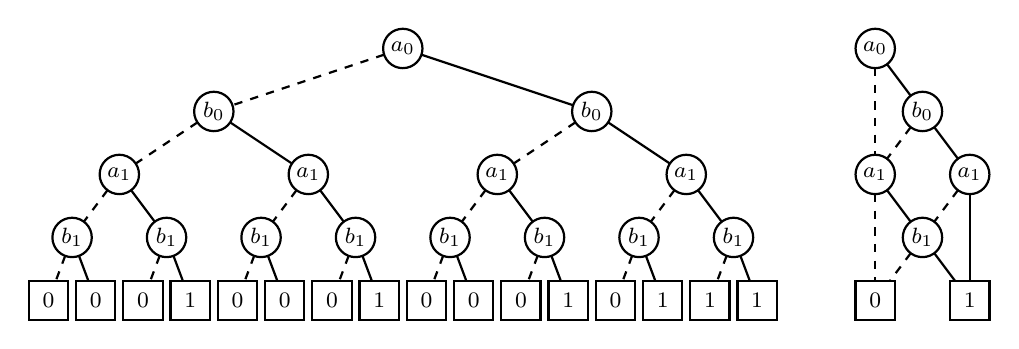
\begin{tikzpicture}
[every node/.style={draw=black,thick,minimum size=5mm,inner sep=0mm,outer sep=0mm,font=\footnotesize},
 var/.style={circle},
 val/.style={rectangle},
 thick]
\node[var] (a0)                                            {$a_0$};
\node[var] (b0A) [on grid,below  left=8mm and 24mm of a0]  {$b_0$};
\node[var] (b0B) [on grid,below right=8mm and 24mm of a0]  {$b_0$};
\node[var] (a1A) [on grid,below  left=8mm and 12mm of b0A] {$a_1$};
\node[var] (a1B) [on grid,below right=8mm and 12mm of b0A] {$a_1$};
\node[var] (a1C) [on grid,below  left=8mm and 12mm of b0B] {$a_1$};
\node[var] (a1D) [on grid,below right=8mm and 12mm of b0B] {$a_1$};
\node[var] (b1A) [on grid,below  left=8mm and  6mm of a1A] {$b_1$};
\node[var] (b1B) [on grid,below right=8mm and  6mm of a1A] {$b_1$};
\node[var] (b1C) [on grid,below  left=8mm and  6mm of a1B] {$b_1$};
\node[var] (b1D) [on grid,below right=8mm and  6mm of a1B] {$b_1$};
\node[var] (b1E) [on grid,below  left=8mm and  6mm of a1C] {$b_1$};
\node[var] (b1F) [on grid,below right=8mm and  6mm of a1C] {$b_1$};
\node[var] (b1G) [on grid,below  left=8mm and  6mm of a1D] {$b_1$};
\node[var] (b1H) [on grid,below right=8mm and  6mm of a1D] {$b_1$};
\node[val] (tA)  [on grid,below  left=8mm and  3mm of b1A] {0};
\node[val] (tB)  [on grid,below right=8mm and  3mm of b1A] {0};
\node[val] (tC)  [on grid,below  left=8mm and  3mm of b1B] {0};
\node[val] (tD)  [on grid,below right=8mm and  3mm of b1B] {1};
\node[val] (tE)  [on grid,below  left=8mm and  3mm of b1C] {0};
\node[val] (tF)  [on grid,below right=8mm and  3mm of b1C] {0};
\node[val] (tG)  [on grid,below  left=8mm and  3mm of b1D] {0};
\node[val] (tH)  [on grid,below right=8mm and  3mm of b1D] {1};
\node[val] (tI)  [on grid,below  left=8mm and  3mm of b1E] {0};
\node[val] (tJ)  [on grid,below right=8mm and  3mm of b1E] {0};
\node[val] (tK)  [on grid,below  left=8mm and  3mm of b1F] {0};
\node[val] (tL)  [on grid,below right=8mm and  3mm of b1F] {1};
\node[val] (tM)  [on grid,below  left=8mm and  3mm of b1G] {0};
\node[val] (tN)  [on grid,below right=8mm and  3mm of b1G] {1};
\node[val] (tO)  [on grid,below  left=8mm and  3mm of b1H] {1};
\node[val] (tP)  [on grid,below right=8mm and  3mm of b1H] {1};
\path[dashed] (a0)  edge (b0A);
\path         (a0)  edge (b0B);
\path[dashed] (b0A) edge (a1A);
\path         (b0A) edge (a1B);
\path[dashed] (b0B) edge (a1C);
\path         (b0B) edge (a1D);
\path[dashed] (a1A) edge (b1A);
\path         (a1A) edge (b1B);
\path[dashed] (a1B) edge (b1C);
\path         (a1B) edge (b1D);
\path[dashed] (a1C) edge (b1E);
\path         (a1C) edge (b1F);
\path[dashed] (a1D) edge (b1G);
\path         (a1D) edge (b1H);
\path[dashed] (b1A) edge (tA);
\path         (b1A) edge (tB);
\path[dashed] (b1B) edge (tC);
\path         (b1B) edge (tD);
\path[dashed] (b1C) edge (tE);
\path         (b1C) edge (tF);
\path[dashed] (b1D) edge (tG);
\path         (b1D) edge (tH);
\path[dashed] (b1E) edge (tI);
\path         (b1E) edge (tJ);
\path[dashed] (b1F) edge (tK);
\path         (b1F) edge (tL);
\path[dashed] (b1G) edge (tM);
\path         (b1G) edge (tN);
\path[dashed] (b1H) edge (tO);
\path         (b1H) edge (tP);
\node[var] (Ra0)  [on grid,right=60 mm of a0]               {$a_0$};
\node[var] (Rb0)  [on grid,below right=8mm and 6mm of Ra0]  {$b_0$};
\node[var] (Ra1A) [on grid,below  left=8mm and 6mm of Rb0]  {$a_1$};
\node[var] (Ra1B) [on grid,below right=8mm and 6mm of Rb0]  {$a_1$};
\node[var] (Rb1)  [on grid,below right=8mm and 6mm of Ra1A] {$b_1$};
\node[val] (R0)   [on grid,below  left=8mm and 6mm of Rb1]  {0};
\node[val] (R1)   [on grid,below right=8mm and 6mm of Rb1]  {1};
\path[dashed] (Ra0)  edge (Ra1A);
\path         (Ra0)  edge (Rb0);
\path[dashed] (Rb0)  edge (Ra1A);
\path         (Rb0)  edge (Ra1B);
\path[dashed] (Ra1A) edge (R0);
\path         (Ra1A) edge (Rb1);
\path[dashed] (Ra1B) edge (Rb1);
\path         (Ra1B) edge (R1);
\path[dashed] (Rb1)  edge (R0);
\path         (Rb1)  edge (R1);
\end{tikzpicture}

\caption{The Boolean function $c_1$ as an OBDD (left) and an ROBDD (right). The solid lines represent high paths and the dashed lines represent low paths.}
\label{fig:bdd_c1}
\end{figure}

\begin{figure}
\centering
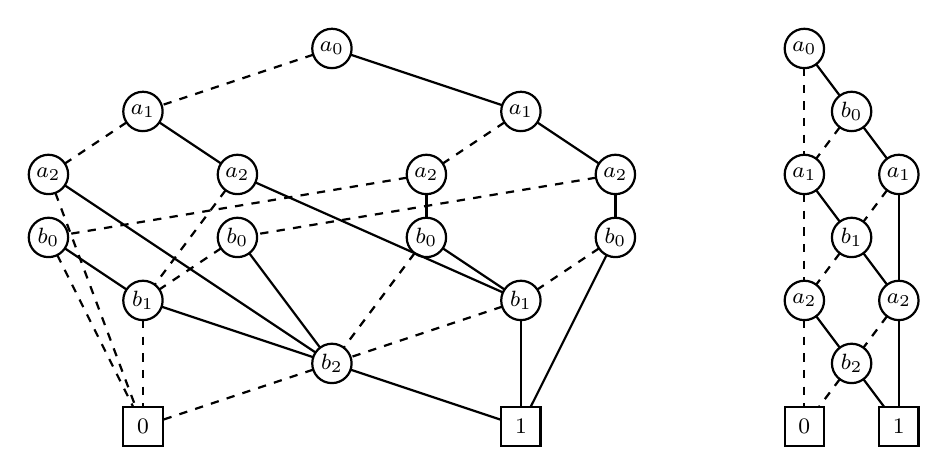
\begin{tikzpicture}
[every node/.style={draw=black,thick,minimum size=5mm,inner sep=0mm,outer sep=0mm,font=\footnotesize},
 var/.style={circle},
 val/.style={rectangle},
 thick]
\node[var] (a0)                                            {$a_0$};
\node[var] (a1A) [on grid,below  left=8mm and 24mm of a0]  {$a_1$};
\node[var] (a1B) [on grid,below right=8mm and 24mm of a0]  {$a_1$};
\node[var] (a2A) [on grid,below  left=8mm and 12mm of a1A] {$a_2$};
\node[var] (a2B) [on grid,below right=8mm and 12mm of a1A] {$a_2$};
\node[var] (a2C) [on grid,below  left=8mm and 12mm of a1B] {$a_2$};
\node[var] (a2D) [on grid,below right=8mm and 12mm of a1B] {$a_2$};
\node[var] (b0A) [on grid,below right=8mm and  0mm of a2A] {$b_0$};
\node[var] (b0B) [on grid,below right=8mm and  0mm of a2B] {$b_0$};
\node[var] (b0C) [on grid,below right=8mm and  0mm of a2C] {$b_0$};
\node[var] (b0D) [on grid,below right=8mm and  0mm of a2D] {$b_0$};
\node[var] (b1A) [on grid,below right=8mm and 12mm of b0A] {$b_1$};
\node[var] (b1B) [on grid,below right=8mm and 12mm of b0C] {$b_1$};
\node[var] (b2)  [on grid,below right=8mm and 24mm of b1A] {$b_2$};
\node[val] (0)   [on grid,below  left=8mm and 24mm of b2]  {0};
\node[val] (1)   [on grid,below right=8mm and 24mm of b2]  {1};
\path[dashed] (a0)  edge (a1A);
\path         (a0)  edge (a1B);
\path[dashed] (a1A) edge (a2A);
\path         (a1A) edge (a2B);
\path[dashed] (a1B) edge (a2C);
\path         (a1B) edge (a2D);
\path[dashed] (a2A) edge (0);
\path         (a2A) edge (b2);
\path[dashed] (a2B) edge (b1A);
\path         (a2B) edge (b1B);
\path[dashed] (a2C) edge (b0A);
\path         (a2C) edge (b0C);
\path[dashed] (a2D) edge (b0B);
\path         (a2D) edge (b0D);
\path[dashed] (b0A) edge (0);
\path         (b0A) edge (b1A);
\path[dashed] (b0B) edge (b1A);
\path         (b0B) edge (b2);
\path[dashed] (b0C) edge (b2);
\path         (b0C) edge (b1B);
\path[dashed] (b0D) edge (b1B);
\path         (b0D) edge (1);
\path[dashed] (b1A) edge (0);
\path         (b1A) edge (b2);
\path[dashed] (b1B) edge (b2);
\path         (b1B) edge (1);
\path[dashed] (b2)  edge (0);
\path         (b2)  edge (1);
\node[var] (Ga0)  [on grid,right=60mm of a0]                {$a_0$};
\node[var] (Gb0)  [on grid,below right=8mm and 6mm of Ga0]  {$b_0$};
\node[var] (Ga1A) [on grid,below  left=8mm and 6mm of Gb0]  {$a_1$};
\node[var] (Ga1B) [on grid,below right=8mm and 6mm of Gb0]  {$a_1$};
\node[var] (Gb1)  [on grid,below right=8mm and 6mm of Ga1A] {$b_1$};
\node[var] (Ga2A) [on grid,below  left=8mm and 6mm of Gb1]  {$a_2$};
\node[var] (Ga2B) [on grid,below right=8mm and 6mm of Gb1]  {$a_2$};
\node[var] (Gb2)  [on grid,below right=8mm and 6mm of Ga2A] {$b_2$};
\node[val] (G0)   [on grid,below  left=8mm and 6mm of Gb2]  {0};
\node[val] (G1)   [on grid,below right=8mm and 6mm of Gb2]  {1};
\path[dashed] (Ga0)  edge (Ga1A);
\path         (Ga0)  edge (Gb0);
\path[dashed] (Gb0)  edge (Ga1A);
\path         (Gb0)  edge (Ga1B);
\path[dashed] (Ga1A) edge (Ga2A);
\path         (Ga1A) edge (Gb1);
\path[dashed] (Ga1B) edge (Gb1);
\path         (Ga1B) edge (Ga2B);
\path[dashed] (Gb1)  edge (Ga2A);
\path         (Gb1)  edge (Ga2B);
\path[dashed] (Ga2A) edge (G0);
\path         (Ga2A) edge (Gb2);
\path[dashed] (Ga2B) edge (Gb2);
\path         (Ga2B) edge (G1);
\path[dashed] (Gb2)  edge (G0);
\path         (Gb2)  edge (G1);
\end{tikzpicture}

\caption{The Boolean function $c_2$ in ROBDD form using the variable order $a_0,a_1,a_2,b_0,b_1,b_2$ (left) and $a_0,b_0,a_1,b_1,a_2,b_2$ (right).}
\label{fig:bdd_c2_bad}
\end{figure}

\chapter{Design}
\label{ch:design}

% machine: registers,flags

\section{...}

\subsection{Flag control}

% stc,clc,cmc

\subsection{Data transfer}

% mov,cmov

\subsection{Logic}

% and,or,xor
% not (one's complement negation)

\subsection{Addition and subtraction}

% add
% adc,sub,sbb,cmp,inc,dec all similar
% neg (two's complement negation): not+inc

\subsection{Multiplication}

% most difficult: multiplication

\chapter{Results}
\label{ch:results}

\chapter{Discussion}
\label{ch:discussion}

\bibliographystyle{ieeetr}
\bibliography{thesis}

\end{document}
